\documentclass[a4paper,11pt]{article}
\usepackage[a4paper, margin=8em]{geometry}

% usa i pacchetti per la scrittura in italiano
\usepackage[french,italian]{babel}
\usepackage[T1]{fontenc}
\usepackage[utf8]{inputenc}
\frenchspacing 

% usa i pacchetti per la formattazione matematica
\usepackage{amsmath, amssymb, amsthm, amsfonts}

% usa altri pacchetti
\usepackage{gensymb}
\usepackage{hyperref}
\usepackage{standalone}

\usepackage{colortbl}

\usepackage{xstring}
\usepackage{karnaugh-map}

% imposta il titolo
\title{Appunti Reti Informatiche}
\author{Luca Seggiani}
\date{2025}

% imposta lo stile
% usa helvetica
\usepackage[scaled]{helvet}
% usa palatino
\usepackage{palatino}
% usa un font monospazio guardabile
\usepackage{lmodern}

\renewcommand{\rmdefault}{ppl}
\renewcommand{\sfdefault}{phv}
\renewcommand{\ttdefault}{lmtt}

% circuiti
\usepackage{circuitikz}
\usetikzlibrary{babel}

% testo cerchiato
\newcommand*\circled[1]{\tikz[baseline=(char.base)]{
            \node[shape=circle,draw,inner sep=2pt] (char) {#1};}}

% disponi il titolo
\makeatletter
\renewcommand{\maketitle} {
	\begin{center} 
		\begin{minipage}[t]{.8\textwidth}
			\textsf{\huge\bfseries \@title} 
		\end{minipage}%
		\begin{minipage}[t]{.2\textwidth}
			\raggedleft \vspace{-1.65em}
			\textsf{\small \@author} \vfill
			\textsf{\small \@date}
		\end{minipage}
		\par
	\end{center}

	\thispagestyle{empty}
	\pagestyle{fancy}
}
\makeatother

% disponi teoremi
\usepackage{tcolorbox}
\newtcolorbox[auto counter, number within=section]{theorem}[2][]{%
	colback=blue!10, 
	colframe=blue!40!black, 
	sharp corners=northwest,
	fonttitle=\sffamily\bfseries, 
	title=Teorema~\thetcbcounter: #2, 
	#1
}

% disponi definizioni
\newtcolorbox[auto counter, number within=section]{definition}[2][]{%
	colback=red!10,
	colframe=red!40!black,
	sharp corners=northwest,
	fonttitle=\sffamily\bfseries,
	title=Definizione~\thetcbcounter: #2,
	#1
}

% disponi codice
\usepackage{listings}
\usepackage[table]{xcolor}

\definecolor{codegreen}{rgb}{0,0.6,0}
\definecolor{codegray}{rgb}{0.5,0.5,0.5}
\definecolor{codepurple}{rgb}{0.58,0,0.82}
\definecolor{backcolour}{rgb}{0.95,0.95,0.92}

\lstdefinestyle{codestyle}{
		backgroundcolor=\color{black!5}, 
		commentstyle=\color{codegreen},
		keywordstyle=\bfseries\color{magenta},
		numberstyle=\sffamily\tiny\color{black!60},
		stringstyle=\color{green!50!black},
		basicstyle=\ttfamily\footnotesize,
		breakatwhitespace=false,         
		breaklines=true,                 
		captionpos=b,                    
		keepspaces=true,                 
		numbers=left,                    
		numbersep=5pt,                  
		showspaces=false,                
		showstringspaces=false,
		showtabs=false,                  
		tabsize=2
}

\lstdefinestyle{shellstyle}{
		backgroundcolor=\color{black!5}, 
		basicstyle=\ttfamily\footnotesize\color{black}, 
		commentstyle=\color{black}, 
		keywordstyle=\color{black},
		numberstyle=\color{black!5},
		stringstyle=\color{black}, 
		showspaces=false,
		showstringspaces=false, 
		showtabs=false, 
		tabsize=2, 
		numbers=none, 
		breaklines=true
}


\lstdefinelanguage{assembler}{ 
  keywords={AAA, AAD, AAM, AAS, ADC, ADCB, ADCW, ADCL, ADD, ADDB, ADDW, ADDL, AND, ANDB, ANDW, ANDL,
        ARPL, BOUND, BSF, BSFL, BSFW, BSR, BSRL, BSRW, BSWAP, BT, BTC, BTCB, BTCW, BTCL, BTR, 
        BTRB, BTRW, BTRL, BTS, BTSB, BTSW, BTSL, CALL, CBW, CDQ, CLC, CLD, CLI, CLTS, CMC, CMP,
        CMPB, CMPW, CMPL, CMPS, CMPSB, CMPSD, CMPSW, CMPXCHG, CMPXCHGB, CMPXCHGW, CMPXCHGL,
        CMPXCHG8B, CPUID, CWDE, DAA, DAS, DEC, DECB, DECW, DECL, DIV, DIVB, DIVW, DIVL, ENTER,
        HLT, IDIV, IDIVB, IDIVW, IDIVL, IMUL, IMULB, IMULW, IMULL, IN, INB, INW, INL, INC, INCB,
        INCW, INCL, INS, INSB, INSD, INSW, INT, INT3, INTO, INVD, INVLPG, IRET, IRETD, JA, JAE,
        JB, JBE, JC, JCXZ, JE, JECXZ, JG, JGE, JL, JLE, JMP, JNA, JNAE, JNB, JNBE, JNC, JNE, JNG,
        JNGE, JNL, JNLE, JNO, JNP, JNS, JNZ, JO, JP, JPE, JPO, JS, JZ, LAHF, LAR, LCALL, LDS,
        LEA, LEAVE, LES, LFS, LGDT, LGS, LIDT, LMSW, LOCK, LODSB, LODSD, LODSW, LOOP, LOOPE,
        LOOPNE, LSL, LSS, LTR, MOV, MOVB, MOVW, MOVL, MOVSB, MOVSD, MOVSW, MOVSX, MOVSXB,
        MOVSXW, MOVSXL, MOVZX, MOVZXB, MOVZXW, MOVZXL, MUL, MULB, MULW, MULL, NEG, NEGB, NEGW,
        NEGL, NOP, NOT, NOTB, NOTW, NOTL, OR, ORB, ORW, ORL, OUT, OUTB, OUTW, OUTL, OUTSB, OUTSD,
        OUTSW, POP, POPL, POPW, POPB, POPA, POPAD, POPF, POPFD, PUSH, PUSHL, PUSHW, PUSHB, PUSHA, 
				PUSHAD, PUSHF, PUSHFD, RCL, RCLB, RCLW, MOVSL, MOVSB, MOVSW, STOSL, STOSB, STOSW, LODSB, LODSW,
				LODSL, INSB, INSW, INSL, OUTSB, OUTSL, OUTSW
        RCLL, RCR, RCRB, RCRW, RCRL, RDMSR, RDPMC, RDTSC, REP, REPE, REPNE, RET, ROL, ROLB, ROLW,
        ROLL, ROR, RORB, RORW, RORL, SAHF, SAL, SALB, SALW, SALL, SAR, SARB, SARW, SARL, SBB,
        SBBB, SBBW, SBBL, SCASB, SCASD, SCASW, SETA, SETAE, SETB, SETBE, SETC, SETE, SETG, SETGE,
        SETL, SETLE, SETNA, SETNAE, SETNB, SETNBE, SETNC, SETNE, SETNG, SETNGE, SETNL, SETNLE,
        SETNO, SETNP, SETNS, SETNZ, SETO, SETP, SETPE, SETPO, SETS, SETZ, SGDT, SHL, SHLB, SHLW,
        SHLL, SHLD, SHR, SHRB, SHRW, SHRL, SHRD, SIDT, SLDT, SMSW, STC, STD, STI, STOSB, STOSD,
        STOSW, STR, SUB, SUBB, SUBW, SUBL, TEST, TESTB, TESTW, TESTL, VERR, VERW, WAIT, WBINVD,
        XADD, XADDB, XADDW, XADDL, XCHG, XCHGB, XCHGW, XCHGL, XLAT, XLATB, XOR, XORB, XORW, XORL},
  keywordstyle=\color{blue}\bfseries,
  ndkeywordstyle=\color{darkgray}\bfseries,
  identifierstyle=\color{black},
  sensitive=false,
  comment=[l]{\#},
  morecomment=[s]{/*}{*/},
  commentstyle=\color{purple}\ttfamily,
  stringstyle=\color{red}\ttfamily,
  morestring=[b]',
  morestring=[b]"
}

\lstset{language=assembler, style=codestyle}

% disponi sezioni
\usepackage{titlesec}

\titleformat{\section}
	{\sffamily\Large\bfseries} 
	{\thesection}{1em}{} 
\titleformat{\subsection}
	{\sffamily\large\bfseries}   
	{\thesubsection}{1em}{} 
\titleformat{\subsubsection}
	{\sffamily\normalsize\bfseries} 
	{\thesubsubsection}{1em}{}

% tikz
\usepackage{tikz}

% float
\usepackage{float}

% grafici
\usepackage{pgfplots}
\pgfplotsset{width=10cm,compat=1.9}

% disponi alberi
\usepackage{forest}

\forestset{
	rectstyle/.style={
		for tree={rectangle,draw,font=\large\sffamily}
	},
	roundstyle/.style={
		for tree={circle,draw,font=\large}
	}
}

% disponi algoritmi
\usepackage{algorithm}
\usepackage{algorithmic}
\makeatletter
\renewcommand{\ALG@name}{Algoritmo}
\makeatother

% disponi numeri di pagina
\usepackage{fancyhdr}
\fancyhf{} 
\fancyfoot[L]{\sffamily{\thepage}}

\makeatletter
\fancyhead[L]{\raisebox{1ex}[0pt][0pt]{\sffamily{\@title \ \@date}}} 
\fancyhead[R]{\raisebox{1ex}[0pt][0pt]{\sffamily{\@author}}}
\makeatother

\begin{document}
% sezione (data)
\section{Lezione del 24-09-25}

% stili pagina
\thispagestyle{empty}
\pagestyle{fancy}

% testo
\subsection{Comunicazione dati su Internet}
Abbiamo visto la struttura a livello fisico della rete Internet.
Vediamo adesso i meccanismi secondo cui la trasmissione di dati avviene.
La rete Internet è una rete a \textbf{commutazione di pacchetto}, il compito degli host è di:
\begin{itemize}
	\item Ottenere messaggi dalle applicazioni;
	\item Dividere quei messaggi in frammenti più piccoli, detti \textbf{pacchetti}, di dimensione $L$ bit;
	\item Trasmettere quei pacchetti nella rete di accesso ad una \textit{frequenza di trasmissione} (o \textbf{bit-rate}) $R$.
\end{itemize}

Il tempo $T_{\text{packet}}$ necessario a trasmettere un pacchetto da $L$ bit su una linea da $R$ bit al secondo di bitrate sarà quindi semplicemente calcolato come:
$$
T_{\text{packet}} = \frac{L}{R}
$$

Il bitrate, detto anche frequenza di \textit{link}, dipende appunto dal \textbf{link} (o \textit{mezzo}) della trasmissione, cioè l'infrastruttura fisica che sta fra trasmettitore e ricevitore.
Possiamo classificare 2 tipi di link:
\begin{itemize}
	\item Mezzi \textbf{guidati}: segnali che si propagano in mezzi solidi (rame, fibra, cavi coassiali, ecc...). 

		\begin{itemize}
			\item 
		Un celebre esempio di mezzo trasmissivo guidato è il classico \textbf{doppino telefonico}, o trasmettitore a \textit{Twisted Pair} (\textbf{TP}). Questo è formato da due fili di rame isolati e avvolti l'uno sull'altro, che permettono la trasmissione differenziale e quindi la riduzione dei rumori in \textit{common-mode};
			\item
		Un altro tipo di mezzo trasmissivo guidato è il \textbf{cavo coassiale}, formato da due conduttori concentrici in rame separati da un dielettrico. Il segnale è trasferito come campo magnetico fra i due conduttori: questo permette bitrate più alti rispetto al normale doppino telefonico e una migliore schermatura dalle interferenze;
			\item
		Infine, possiamo parlare della \textbf{fibra ottica}, formata da fibra di vetro che porta impulsi luminosi ad altissima velocità. Questa tecnologia presenta velocità di trasmissione estremamente alte, e vista la natura luminosa del segnale, non è suscettibile ad interferenze (alta affidabilità, cioè piccola frequenza di errore sui bit).
		\end{itemize}

	\item Mezzi \textbf{non guidati}: segnali che si propagano nell'etere (segnali radio, ecc...). Questi sono solitamente meno sicuri ma significativamente più comodi per l'utente finale (possibilità di spostarsi, mancanza di cavi, ecc...).

		La trasmissione wireless è suscettibile a fenomeni fisici come \textit{riflessi}, \textit{interferenze} e \textit{ostruzione} da parte di oggetti fisici.

		\begin{itemize}
			\item Il \textbf{WiFi} è un esempio di mezzo di trasmissione non guidato che può raggiungere centinaia di Mbps su regioni locali;
			\item Reti wireless più ampie possono essere quelle \textbf{cellulari}, usate nella telefonia mobile;
			\item Infine si può parlare delle \textbf{reti satellitari}, usate per l'interconnessione di regioni geografiche fra di loro anche molto distanti.
		\end{itemize}

\end{itemize}

\subsubsection{Commutazione di circuito}
Prima della commutazione di pacchetto si usava la tecnica della \textbf{commutazione di circuito} (ad esempio sulle linee telefoniche).
Questo prevede di dedicare completamente una certa linea di trasmissione alla comunicazione fra due host, invalidandone quindi l'uso da parte di altri host.

Chiaramente, la commutazione di pacchetto permette un carico migliore della linea, dove più pacchetti provenienti da diverse fonti possono viaggiare a istanti temporali molto vicini fra di loro.

In particolare, la commutazione di paccheto è utile per dati trasmessi in \textit{burst}, mentre la rete a commutazione di circuito assicura minima congestione possibile a costo di occupazione completa della linea.

\subsubsection{Commutazione di pacchetto}
La tecnica della \textbf{commutazione di pacchetto} o \textit{packet-switching} permette ad una rete di \textbf{router} interconnessi di ricevere ed instradare (letteralmente, \textit{"routing"}) pacchetti provenienti da più fonti in modo che raggiungano la loro destinazione.

Questo inserisce chiaramente un ritardo nel sistema, in quanto il router deve:
\begin{itemize}
	\item Ricevere il pacchetto \textit{completamente} ed memorizzarlo: questo richiede $L/R$ secondi;
	\item Leggere l'header del pacchetto per capire il prossimo passo dell'instradamento;
	\item Trasmettere il pacchetto verso la sua nuova destinazione (un altro router o l'host finale), impeigando ancora $L/R$ secondi.
\end{itemize}

Abbiamo quindi che il ritardo end-end immesso dal router è necessariamente di almeno $2L/R$ secondi, tralasciando il tempo necessario all'instradamento stesso. 

Nel caso generale si abbiano $N$ router (quindi $N + 1$ link fra i router) e $P$ pacchetti da inviare, dovremo considerareche il primo pacchetto arriva in $(N + 1) \frac{L}{R}$ (deve attraversare tutti i link) e i successivi $P - 1$ pacchetti arrivano in $(P - 1) \frac{L}{R}$, per cui il tempo complessivo è:
$$
T_{end-to-end} = (N + P) \frac{L}{R}
$$

Se troppi pacchetti arrivano in un breve lasso di tempo, cioè se la frequenza di arrivo supera quella di trasmissione:
\begin{itemize}
	\item I pacchetti verrano messi in coda finché non sarà possibile trasmetterli;
	\item I pacchetti possono essere persi se il buffer di memoria dedicato alla loro memorizzazione nel ruoter si riempie.
\end{itemize}

\subsection{Prestazioni della commutazione di pacchetto}
Facciamo qualche considerazione ulteriore sulle prestazioni delle linee a commutazione di pacchetto.
Abbiamo ottenuto il valore $T_{\text{packet}} = \frac{L}{R}$ per la trasmissione di un singolo pacchetto da $L$ bit su una linea con bitrate $R$, e $T_{\text{end-to-end}} = (N + P) \frac{L}{R}$ per più pacchetti su un numero arbitrario di router.

Da quanto abbiamo detto nella scorsa sezione, un modello più sofisticato del packet-switching terrà conto di 4 sorgenti di ritardo:
\begin{itemize}
	\item Ritardo di \textbf{trasmissione} $T_{\text{trans}}$, dato dalle caratteristiche del link. Come abbiamo già detto, questo vale:
		$$
		T_{\text{trans}} = \frac{L}{R}
		$$
		con $L$ lunghezza del pacchetto in bit e $R$ bitrate del link;
	\item Ritardo di \textbf{propagazione} $T_{\text{prop}}$, dato dalle proprietà fisiche del mezzo di trasmissione. In particolare, questo è il tempo fisico di trasmissione del segnale su un link, dato da:
		$$
		T_{\text{prop}} = \frac{d}{s}
		$$
con $d$ distanza del link e $s$ velocità del mezzo di trasmissione. Chiaramente, per i nostri scopi $s$ sara una frazione significativa della velocità della luce $c \approx 3 \cdot 10^8$ m/s;
	\item Ritardo di \textbf{laborazione} (instradamento) $T_{\text{proc}}$, dipende dalle caratteristiche del router ed è perlopiù costante;
	\item Ritardo di \textbf{accodamento} dato dalla presenza di code $T_{\text{queue}}$. Questo è il più complicato da trattare, in quanto dipende dal numero di pacchetti presenti nel buffer del router. Come vedremo fra poco, una buona euristica per la valutazione di questo ritardo (che è comunque trattabile solo in maniera statistica) è l'\textit{intensità di traffico} sulla linea di trasmissione.
\end{itemize}
Sommando queste sorgenti di ritardo potremo ottenere una stima del ritardo complessivo su un router (nodo) $T_{\text{node}}$:
$$
T_{\text{node}} = T_{\text{trans}} + T_{\text{prop}} + T_{\text{proc}} + T_{\text{queue}}
$$

Dati $N$ nodi e $P$ pacchetti, il ritardo end-to-end potrà quindi essere calcolato semplicemente come:
$$
T_{\text{end-to-end}} = (N + P) T_{\text{node}}
$$

\subsubsection{Ritardo di accodamento}
Come anticipato, possiamo valutare statisticamente il ritardo di accodamento $T_{\text{queue}}$ calcolando l'\textit{intensità di traffico} su una linea:
$$
I_{\text{traffic}} = \frac{L \alpha}{R}
$$
presa $\alpha$ come la frequenza media di trasmissione di pacchetti sull'istante temporale.

Semplicemente tracciando la funzione si nota che se $I_{\text{traffic}} >= 1$ il tempo di di accodamento tende a infinito (si ha necessariamente perdita di pacchetti), per cui vorremo mantenere $I_{\text{traffic}} < 1$, e idealmente $I_{\text{traffic}} << 1$.

\begin{center}
	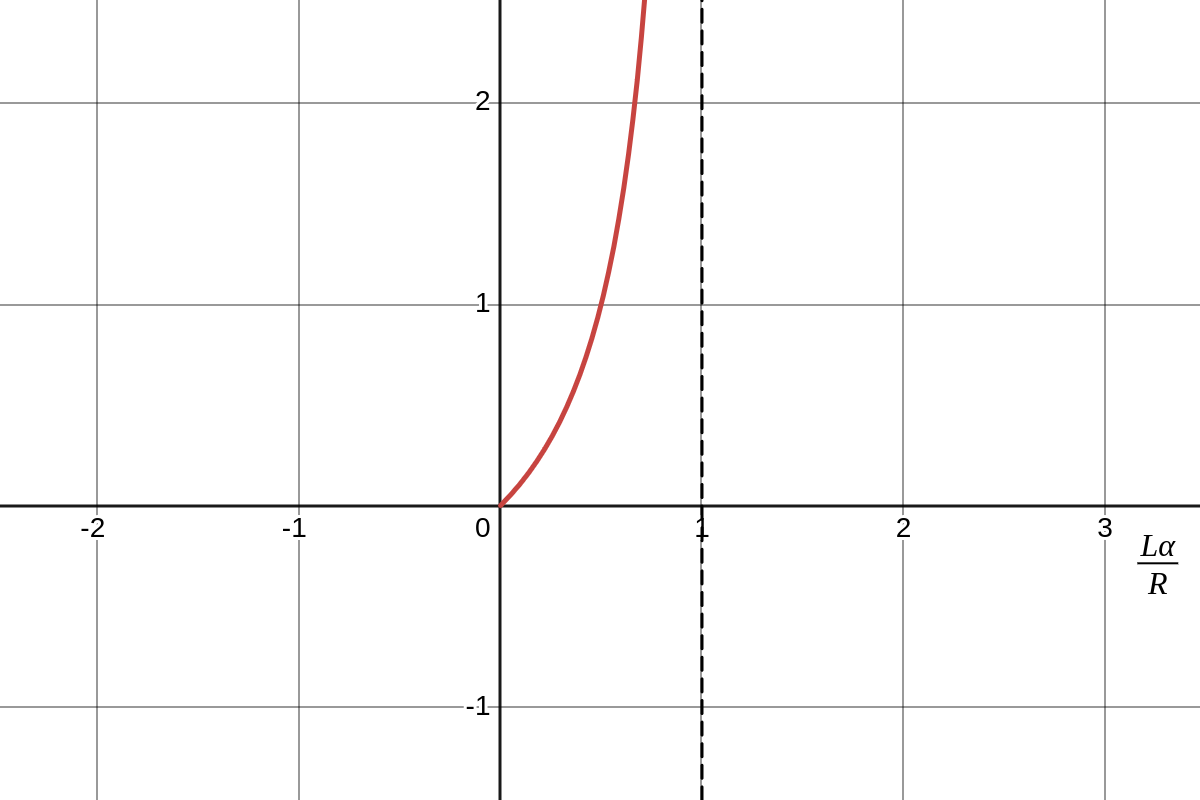
\includegraphics[scale=0.3]{../figures/traf_intensity.png}
\end{center}

\subsubsection{Traceroute}
Per fare diagnostica in situazioni reali, si possono usare software di \textbf{traceroute}, che inviano pacchetti con lo scopo di tracciare gli host incontrati e misurare il tempo impiegato nella trasmissione \textit{round-trip}, o almeno capire se i pacchetti sono stati inviati o persi.

Più nello specifico, ipotizziamo di avere $N$ router fra sorgente e destinazione.
Traceroute invierà $N + 1$ pacchetti speciali sulla linea fra sorgente e destinazione, e ogni router reinvierà il primo di questo che riceve (l'$n$-esimo) indietro alla sorgente, assieme a informazioni temporali e il suo indirizzo.
In questo modo, l'$N + 1$ pacchetto arriverà effettivamente alla destinazione, mentre gli $N$ pacchetti precedenti scandaglieranno ognuno dei router sulla via per la destinazione.

In verità, questo procedimento viene ripetuto 3 volte, per avere risultati più accurati.

Vediamo ad esempio il traceroute che dal portatile su cui sto scrivendo gli appunti arriva ai server dell'Università di Pisa:
\begin{lstlisting}[style=shellstyle]
$ traceroute www.unipi.it
traceroute to www.unipi.it (131.114.104.6), 30 hops max, 60 byte packets
 1  _gateway (10.178.37.4)  3.745 ms  3.552 ms  3.494 ms
 2  172.16.133.129 (172.16.133.129)  300.183 ms  300.156 ms  300.133 ms
 3  172.16.133.38 (172.16.133.38)  60.081 ms  59.673 ms  60.235 ms
 4  172.16.17.50 (172.16.17.50)  52.910 ms  60.413 ms  59.354 ms
 5  151.7.56.70 (151.7.56.70)  61.571 ms  62.259 ms  60.645 ms
 6  151.7.56.66 (151.7.56.66)  89.876 ms  55.029 ms  86.501 ms
 7  151.6.3.199 (151.6.3.199)  52.064 ms 151.6.1.27 (151.6.1.27)  51.777 ms 151.6.3.199 (151.6.3.199)  44.325 ms
 8  151.6.5.139 (151.6.5.139)  52.076 ms 151.6.1.213 (151.6.1.213)  52.842 ms 151.6.5.139 (151.6.5.139)  52.399 ms
 9  garr.rom.namex.it (193.201.28.15)  52.662 ms  51.836 ms  52.516 ms
10  re1-rm02-rs1-rm02.rm02.garr.net (185.191.181.70)  52.317 ms  52.470 ms  52.278 ms
11  rs1-rm02-rs1-pi01.pi01.garr.net (185.191.181.34)  56.893 ms  56.872 ms  56.526 ms
12  rs1-pi01-rl1-pi01.pi01.garr.net (185.191.181.39)  56.495 ms  49.338 ms  50.169 ms
13  rl1-pi01-ru-unipi.pi01.garr.net (193.206.136.90)  49.919 ms  49.808 ms  50.003 ms
14  jser-jspg.unipi.it (131.114.191.90)  51.377 ms  50.215 ms  51.243 ms
15  * * *
16  * * *
17  * * *
18  * * *
19  * * *
20  * * *
21  * * *
22  * * *
23  * * *
24  * * *
25  * * *
26  * * *
27  * * *
28  * * *
29  * * *
30  * * *
\end{lstlisting}
I numeri a sinistra indicano l'indice del router raggiunto, seguiti dall'indirizzo e le misurazioni temporali nei 3 tentativi effettuati dal traceroute.
In praticolare, notiamo come i router da 2 a 8 sono anonimi, al 9 siamo arrivati nella rete del \textit{GARR}, e dal router 15 in poi non abbiamo più ottenuto risposte ai pacchetti traceroute (probabilmente per via della configurazione dei router, il traffico passa comunque).

\subsubsection{Troughput}
Introduciamo il concetto di \textbf{troughput} come la frequenza (bit al secondo) con cui i bit vengono spediti da trasmettitore a ricevitore.
Il throughput può essere:
\begin{itemize}
	\item \textbf{Istantaneo}: calcolato ad un certo istante temporale (per quanto possibile dalla natura discreta della trasmissione);
	\item \textbf{Medio}: calcolato su un periodo temporale più lungo.
\end{itemize}

Ipotizziamo che un server debba inviare un file di $F$ bit ad un client.
La linea di comunicazione fra server e router ha capacità di link di $R_S$ bit/secondo, mentre la linea fra router e client ha capacità di $R_C$ bit/secondo.
Chiaramente la capacità totale sarà:
$$
R_F = \min(R_S, R_C)
$$
cioè link con basse capacità di trasmissione rappresentano \textit{bottleneck} per il throughput di tutto il collegamento fra dispositivi.

\par\smallskip

Facciamo adesso l'esempio di una rete condivisa fra più coppie client/server.
In questo caso, date $N$ coppie, la capacità della rete di interconnessione agli occhi di una singola coppia sarà, preso $R$ come la capacità complessiva:
$$
R_i = \frac{R}{N}
$$
per cui ogni coppia vedrà una linea di comunicazione con capacità:
$$
R_F = \min(R_S, R_C, \frac{R}{N})
$$

\subsection{Struttura di Internet}
Abbiamo detto che Internet è una rete di reti.
\begin{itemize}
	\item Gli host si collegano a internet attraverso le \textit{reti di accesso} (reti LAN, istituzionali, reti mobili, ecc...);
	\item Le reti di accesso si collegano agli \textbf{ISP} (\textit{Internet Server Provider});
	\item Gli ISP devono essere collegati ad altri ISP per permettere la comunicazione fra host su diversi ISP (all'interno di \textbf{IXP} (\textit{Internet eXchange Point}, ecc...)).
\end{itemize}

La struttura di reti interconnesse che si viene a formare è molto complessa, e la sua evoluzione è stata guidata da fattori economici e politici.

Abbiamo quindi una struttura gerarchica:
\begin{enumerate}
	\item Al livello più alto troviamo i cosiddetti \textbf{tier 1 ISP} e i \textbf{content provider} (Google, Facebook, ecc...) che si occupano di copertura nazionale e internazionale. In particolare, i content provider preferiscono collegarsi direttamente agli IXP per risparmiare sugli ISP;
	\item Seguono gli \textbf{IXP}, che collegano più ISP fra di loro, e gli ISP locali (regionali, ecc...);
	\item Infine troviamo le reti di 	\textbf{accesso} locale (reti LAN, WLAN, ecc...).
\end{enumerate}

\subsection{Sicurezza Internet}
La struttura di Internet espone i suoi utenti a diversi pericoli, fra cui:
\begin{itemize}
	\item \textbf{Virus}: programmi maligni che si replicano modificando altri programmi;
	\item \textbf{Worm}: programmi maligni che si replicano con lo scopo di diffondersi in altri computer;
	\item \textbf{Spyware}: programmi maligni che cercano di ottenere informazioni che violano la privacy;
\end{itemize}
ed altre svariate categorie di \textit{malware}.

\subsubsection{Attacchi DoS}
Un caso tipico di attacchi informatici in rete è quello degli attacchi \textbf{DoS} (\textit{Denial of Service}), dove l'attaccante cerca di sfruttare le risorse di un server (memoria, larghezza di banda) al punto di renderlo inutilizzabile ad altri utente.
Questo può essere fatto inviando traffico maligno al server (pacchetti molto grandi o corrotti).

La tecnica può essere espansa a più attaccanti (\textit{botnet}) dando vita a tecniche più sofisticate (come il \textbf{DDoS}, \textit{Distributed Denial of Service}).

\subsubsection{Intercezione di pacchetti}
Una problematica delle reti a commutazione di pacchetto è l'\textbf{intercezione} dei pacchetti instradati, o in inglese \textit{packet sniffing}.
Questo è più facile su reti wireless piuttosto che cablate, ed espone pericoli ovvi per la sicurezza (password, dati sensibili, ecc...).

Oggi, come vedremo, si usano protocolli che implementano forme di crittografia per mitigare questo tipo di problematiche.

\subsubsection{Spoofing IP}
Il problema di identità fasulle si presenta in Internet attraverso pacchetti malformati, con indirizzi sorgente sbagliati. 
Queste tecniche, seppure meno pericolose, possono comunque essere usate per confondere o comunque complicare il traffico sulle reti.

\end{document}
